\documentclass[11pt]{article}

\usepackage[margin=1in]{geometry}
\usepackage[T1]{fontenc}
\usepackage[utf8]{inputenc}
\usepackage{lmodern}
\usepackage{amsmath, amssymb}
\usepackage{booktabs}
\usepackage{graphicx}
\usepackage{float}
\usepackage{hyperref}
\usepackage[numbers]{natbib}

\title{RL for Bilateral Price Negotiation}
\author{Final Project Team\\The Chinese University of Hong Kong, Shenzhen}
\date{April 29, 2026}

\begin{document}

\maketitle

\begin{abstract}
We study bilateral price negotiation as a reinforcement learning problem for large language models. The task is a private-value bargaining game in which a buyer tries to purchase below a hidden budget and a seller tries to sell above a hidden cost, while both sides must keep private values secret and obey a strict action grammar. We build a rule-generated negotiation environment, initialize the policy from supervised fine-tuning, and then optimize negotiation behavior with a three-stage Group Relative Policy Optimization (GRPO) pipeline over role-specific LoRA adapters. The main technical contribution is a training setup that keeps buyer and seller updates separate even though they share one base model, plus a balanced reward that discourages one-sided bargaining equilibria. On held-out rollouts, the best final variant (V1) reaches an 86\% deal rate over 50 validation scenarios with zero format errors and positive reward for both roles. We also report negative results: stronger guardrails in later variants improve some qualitative behaviors but reduce deal quality and stability. The project shows that reward design, opponent choice, and role separation matter as much as language modeling when RL is applied to negotiation.
\end{abstract}

\section{Introduction}

Negotiation is a natural testbed for reinforcement learning because the quality of a response depends on its long-horizon interactive consequences, not just local fluency. In this project, we focus on second-hand marketplace bargaining, where two agents exchange offers until they reach a deal or walk away. The challenge is not only to speak naturally, but also to optimize price, respect role-specific constraints, and avoid leaking private information.

The core motivation for RL is that supervised fine-tuning (SFT) can teach formatting and conversational style, but it cannot directly optimize strategic outcomes such as deal price, legality, or balanced surplus. We therefore treat each negotiation as an episodic environment and train with GRPO, a relative policy optimization method that compares samples inside a rollout group rather than relying on a learned value function \citep{shaobing2024deepseekmath}. Our implementation starts from a Qwen2.5-3B-Instruct base model adapted by SFT, then adds two role-specific LoRA adapters \citep{qwen2025technicalreport,hu2022lora}.

This report is organized around the course grading rubric: problem formulation, method, experiments and results, writing clarity, and novelty. We make four main claims:
\begin{enumerate}
    \item bilateral negotiation can be cast as a reproducible RL environment with explicit terminal outcomes and rule-based rewards;
    \item role-specific adapters are necessary because buyer and seller objectives are fundamentally opposed;
    \item a staged curriculum is more stable than fully joint optimization from the start;
    \item stronger behavioral constraints are not automatically better, because they can damage deal rate and economic utility even when they improve qualitative behavior.
\end{enumerate}

\section{Problem Formulation}

\subsection{Task Definition}

Each scenario describes a used item with three key values: buyer budget $b$, seller cost $c$, and a public market reference price. The buyer should buy below $b$, the seller should sell above $c$, and neither side should reveal its private threshold. The dialogue must use one of three parser-compatible actions:
\begin{itemize}
    \item an offer such as \texttt{[PRICE: 1220]};
    \item a commitment action such as \texttt{<deal>1220</deal>};
    \item a refusal action \texttt{<walkaway>}.
\end{itemize}

The environment terminates in one of five outcomes: legal deal, buyer violation, seller violation, walkaway, timeout, or format error. A legal deal must satisfy $c \le p \le b$ for the final agreed price $p$.

\subsection{Why RL Is Appropriate}

The final quality of a negotiation policy depends on interactive outcomes rather than one-step labels. A buyer that speaks fluently but accepts the seller's first anchor at its full budget is not a good negotiator. Likewise, a seller that produces realistic language but agrees below cost is strategically useless. RL is therefore a better fit than pure SFT because it can directly optimize:
\begin{itemize}
    \item economic utility of the final deal;
    \item legality of the outcome;
    \item walkaway decisions under failed bargaining;
    \item absence of private-value leakage;
    \item multi-turn behavior such as gradual concession.
\end{itemize}

\subsection{Scenario Difficulty}

We control difficulty through the bargaining zone:
\begin{equation}
    \text{gap\_ratio} = \frac{b-c}{c}.
\end{equation}

Small values of $\text{gap\_ratio}$ create near-zero-surplus scenarios, while larger values create wider bargaining zones. The RL dataset intentionally emphasizes harder cases. The generated split is shown in Table~\ref{tab:data-distribution}.

\begin{table}[H]
\centering
\caption{Rule-generated RL scenario distribution.}
\label{tab:data-distribution}
\begin{tabular}{lccccc}
\toprule
Split & Total & Near-zero & Narrow & Balanced & Wide \\
\midrule
Train & 4000 & 1008 & 1426 & 980 & 586 \\
Validation & 500 & 114 & 163 & 139 & 84 \\
Test & 500 & 118 & 193 & 124 & 65 \\
\bottomrule
\end{tabular}
\end{table}

\section{Method}

\subsection{From SFT to Online GRPO}

Our training pipeline has two phases. First, SFT teaches the model the negotiation language: role identity, action syntax, deal and walkaway patterns, and a plausible multi-turn rhythm. The SFT data is synthesized from rule-generated scenarios and converted into turn-level messages. This stage is necessary for stable parsing, but it is not enough for strategic quality.

Second, we switch to online self-play with GRPO. For each scenario, the current policies generate a full trajectory, the environment parses the terminal outcome, and the system computes role-specific reward. GRPO then normalizes rewards within a sampled group and updates only the active role adapter. Relative optimization is attractive here because negotiation outcomes are sparse and highly scenario-dependent.

\subsection{Role-Specific Adapters}

The base model is a merged SFT checkpoint built on Qwen2.5-3B-Instruct. We attach two LoRA adapters:
\begin{align}
    \pi_{\text{buyer}} &= \text{BaseModel} + \text{BuyerAdapter}, \\
    \pi_{\text{seller}} &= \text{BaseModel} + \text{SellerAdapter}.
\end{align}

This design lets both roles share the same linguistic backbone while keeping their updates separate. A single shared adapter would make the reward signal inconsistent because buyer and seller utilities point in opposite directions on the same trajectory.

\subsection{Reward Design}

For legal deals, we normalize utility by the bargaining zone:
\begin{align}
    u_{\text{buyer}} &= \frac{b-p}{b-c}, \\
    u_{\text{seller}} &= \frac{p-c}{b-c}.
\end{align}

The environment uses these utilities as the main terminal reward, scaled to a 100-point range. It also adds shaping terms and penalties for:
\begin{itemize}
    \item invalid deals above the buyer budget or below the seller cost;
    \item format errors and missing parser targets;
    \item private-value leakage such as claiming a floor price or maximum budget;
    \item extreme offers far outside the market range;
    \item non-monotone concession behavior.
\end{itemize}

The most important reward innovation is the balanced stage-3 variant V1, which mixes each role's own terminal reward with a shared Nash-style term:
\begin{equation}
    r_{\text{shared}} = \sqrt{u_{\text{buyer}} \cdot u_{\text{seller}}}.
\end{equation}
This reward does not force identical utilities, but it discourages collapse into one-sided equilibria where one role captures almost all surplus.

\subsection{Three-Stage Curriculum}

We found a staged curriculum more stable than directly updating both roles together:
\begin{enumerate}
    \item \textbf{Stage 1}: train the buyer against a frozen seller;
    \item \textbf{Stage 2}: train the seller against a frozen buyer;
    \item \textbf{Stage 3}: alternate buyer and seller updates with a lower learning rate and KL regularization.
\end{enumerate}

The key hyperparameters are listed in Table~\ref{tab:training-stages}.

\begin{table}[H]
\centering
\caption{Training stages and representative hyperparameters.}
\label{tab:training-stages}
\begin{tabular}{lllll}
\toprule
Stage & Active role & LR & KL $\beta$ & Notes \\
\midrule
1 & Buyer & $5\times10^{-6}$ & 0.04 & Seller frozen, cold-seller guard \\
2 & Seller & $5\times10^{-6}$ & 0.04 & Buyer frozen \\
1.2 & Buyer & $3\times10^{-6}$ & 0.06 & Buyer retrained against stronger seller \\
3 & Alternating & $1\times10^{-6}$ to $7\times10^{-7}$ & 0.08 to 0.10 & Buyer and seller update in turn \\
\bottomrule
\end{tabular}
\end{table}

\subsection{Implementation Details}

The project uses LoRA rank 64, LoRA alpha 128, dropout 0.05, rollout group size 8, at most 10 rounds per negotiation, and a completion limit of 96 tokens. The action history is parsed online and the environment immediately terminates on illegal or malformed actions. During stage 3, gradient accumulation is tracked per adapter rather than globally; otherwise buyer and seller optimizer steps can become misaligned when roles alternate.

\section{Experiments}

\subsection{Evaluation Questions}

We evaluate the system with four practical questions:
\begin{enumerate}
    \item Can the model reach legal deals reliably?
    \item Are rewards positive for both roles, rather than collapsing to one-sided wins?
    \item Do later reward constraints improve qualitative behavior?
    \item Which stage-2 seller checkpoint is the best opponent for buyer retraining?
\end{enumerate}

\subsection{Metrics}

We report deal rate, violation rates, walkaway rate, format error rate, average buyer reward, average seller reward, and average number of rounds. For some analyses, we also compute buyer surplus share and price-to-budget ratio. These metrics cover both strategic success and safety/format behavior.

\subsection{Ablations}

We use two main ablation families:
\begin{itemize}
    \item \textbf{Stage-2 seller checkpoint comparison}: compare \texttt{\_init}, \texttt{step\_50}, \texttt{best}, \texttt{step\_100}, and \texttt{final} seller adapters while keeping the buyer fixed.
    \item \textbf{Stage-3 reward variants}: compare V1, V2, and V3 final policies, where V1 introduces shared balance reward and V2/V3 add stronger behavior constraints.
\end{itemize}

\section{Results}

\subsection{Choosing the Seller for Buyer Retraining}

The first negative result came from stage 3: a strong seller could drive the system toward near-budget deals that left the buyer with almost no surplus. To fix this, we compared multiple stage-2 seller checkpoints as frozen opponents for stage 1.2 buyer retraining. Results are in Table~\ref{tab:seller-ckpt}.

\begin{table}[H]
\centering
\caption{Stage-2 seller checkpoint comparison against the same frozen buyer.}
\label{tab:seller-ckpt}
\begin{tabular}{lcccc}
\toprule
Seller checkpoint & Legal deal rate & Buyer reward & Seller reward & Buyer surplus share \\
\midrule
\texttt{\_init\_seller} & 62.5\% & 13.20 & 39.53 & 0.190 \\
\texttt{step\_50} & 96.9\% & 6.13 & 94.51 & 0.043 \\
\texttt{best} & 96.9\% & 3.07 & 96.40 & 0.000 \\
\texttt{step\_100} & 96.9\% & 23.93 & 95.28 & 0.129 \\
\texttt{final} & 90.6\% & 24.51 & 82.07 & 0.172 \\
\bottomrule
\end{tabular}
\end{table}

The \texttt{best} seller checkpoint was too dominant: it achieved a high legal-deal rate, but the buyer captured essentially no surplus. We therefore selected \texttt{step\_100} as the default frozen opponent for stage 1.2 because it preserved strong deal quality while leaving room for buyer learning.

\subsection{Stage-3 Training Behavior}

Figure~\ref{fig:reward-curves} shows the training-time evaluation curves for the three stage-3 variants. V1 is the strongest overall variant. It delivers the highest and most stable reward signal while keeping both roles viable. V2 and V3 add heavier guardrails against leakage, unfair early deals, and low-utility acceptance, but these constraints make optimization harder.

\begin{figure}[H]
\centering
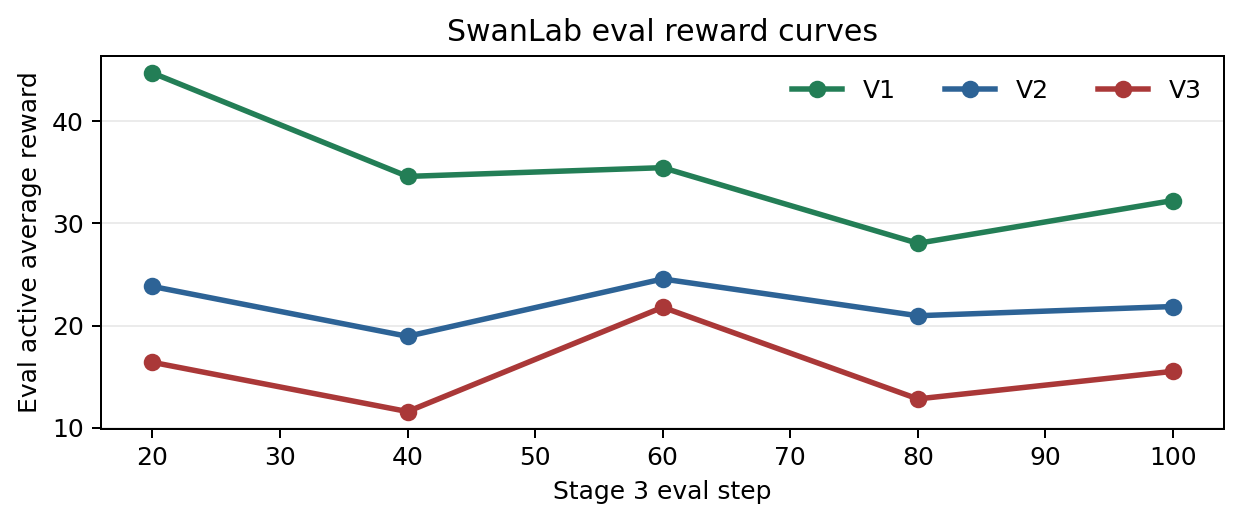
\includegraphics[width=0.9\linewidth]{figures/swanlab_reward_curve.png}
\caption{SwanLab evaluation reward curves for the three stage-3 variants. V1 converges most cleanly; V2 and V3 are less stable under stronger constraints.}
\label{fig:reward-curves}
\end{figure}

The richer SwanLab metrics make the trade-off more explicit. Figure~\ref{fig:stage3-dynamics} shows that V2 and V3 produce longer dialogues but still underperform V1 on deal rate and seller violation rate. Figure~\ref{fig:stage3-balance} shows why this matters: V1 is the only variant that keeps the seller's raw reward consistently positive while reducing the buyer-seller reward gap over training.

\begin{figure}[H]
\centering
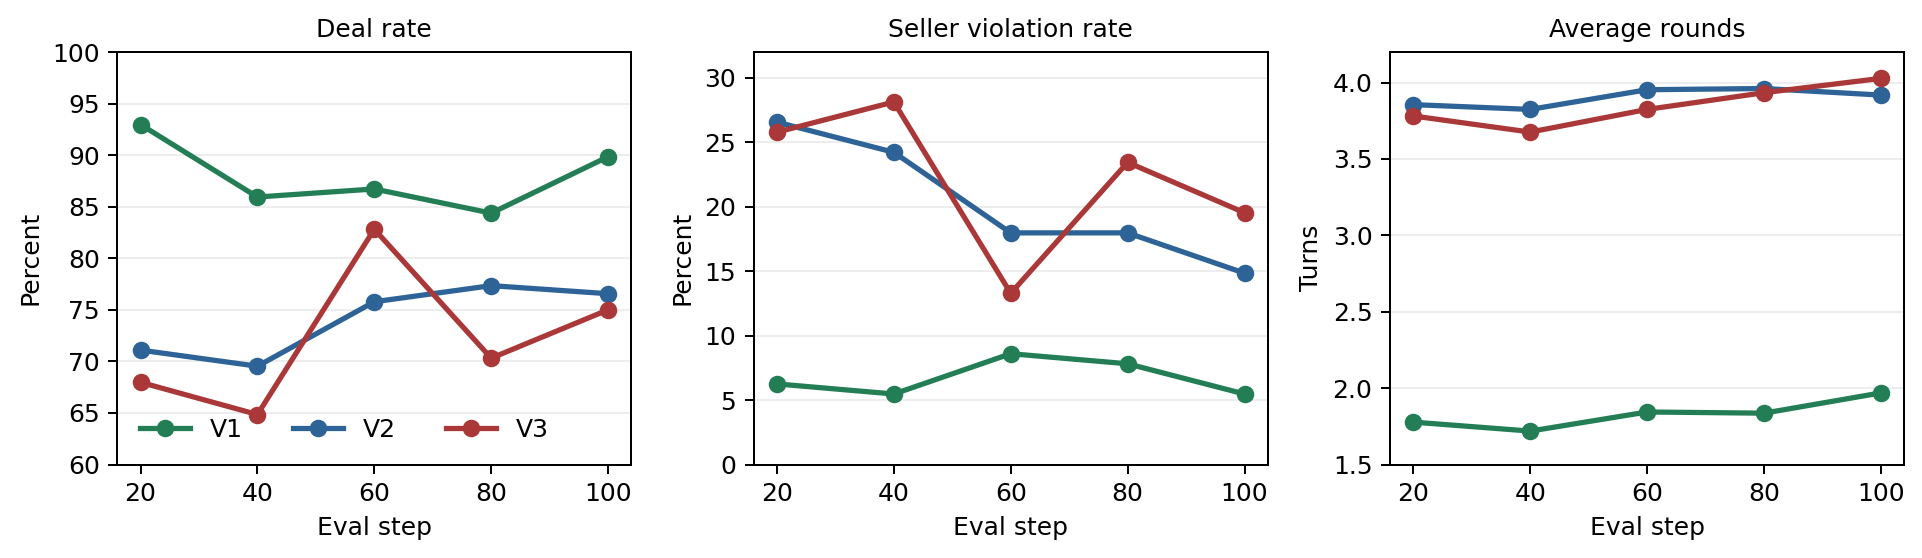
\includegraphics[width=\linewidth]{figures/swanlab_stage3_dynamics.png}
\caption{Stage-3 dynamics from SwanLab. Heavier guardrails lead to longer dialogues, but they do not recover V1's deal rate or low seller-violation behavior.}
\label{fig:stage3-dynamics}
\end{figure}

\begin{figure}[H]
\centering
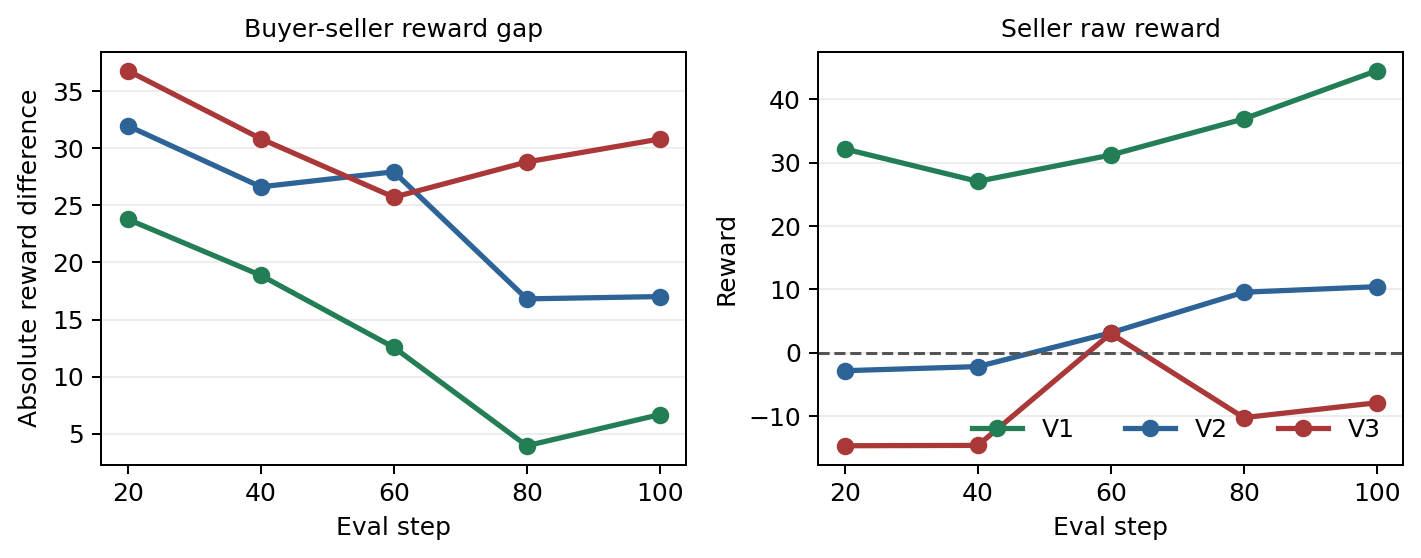
\includegraphics[width=0.92\linewidth]{figures/swanlab_stage3_balance.png}
\caption{Balance diagnostics from SwanLab. V1 narrows the buyer-seller reward gap while keeping seller reward above zero; V2 and V3 often push seller reward to zero or below.}
\label{fig:stage3-balance}
\end{figure}

\subsection{Final Policy Comparison}

The final policy comparison on 15 held-out scenarios is summarized in Table~\ref{tab:v123-final}. V1 is the clear winner on aggregate quality.

\begin{table}[H]
\centering
\caption{Final policy ablation over 15 held-out scenarios.}
\label{tab:v123-final}
\begin{tabular}{lcccccc}
\toprule
Variant & Deal rate & Buyer viol. & Seller viol. & Walkaway & Buyer reward & Seller reward \\
\midrule
V1 & 100.0\% & 0.0\% & 0.0\% & 0.0\% & 23.48 & 59.45 \\
V2 & 73.3\% & 0.0\% & 13.3\% & 13.3\% & 12.37 & 24.78 \\
V3 & 73.3\% & 6.7\% & 20.0\% & 0.0\% & 4.17 & 20.40 \\
\bottomrule
\end{tabular}
\end{table}

We repeated the comparison on a larger 50-scenario sample for V1 and two V3 checkpoints. Figure~\ref{fig:v123-ablation} and Table~\ref{tab:larger-ablation} tell the same story: V1 remains the best trade-off between legal deal rate and two-sided utility.

\begin{figure}[H]
\centering
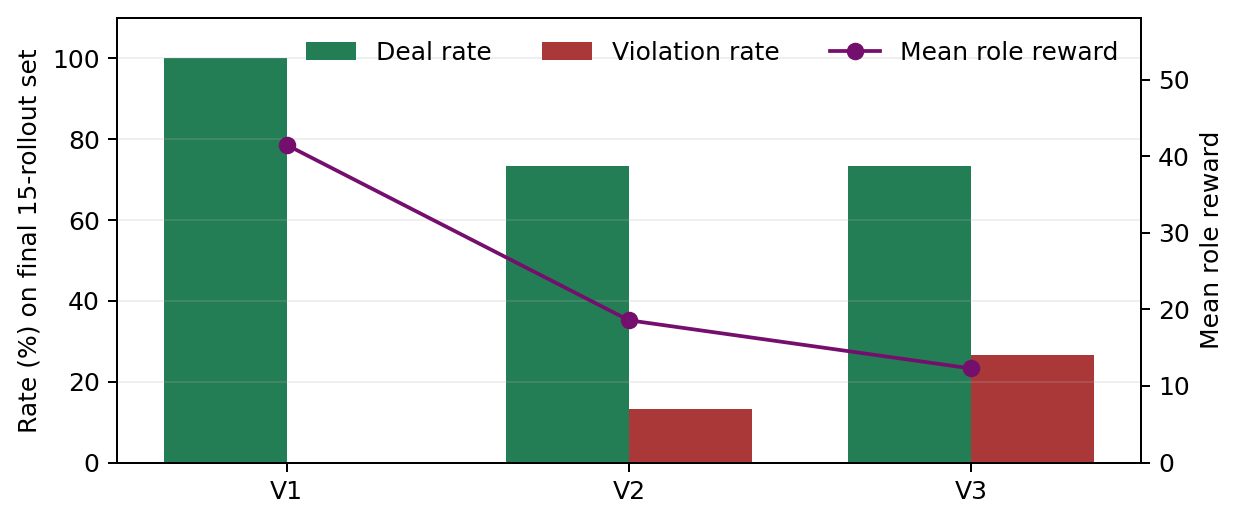
\includegraphics[width=0.85\linewidth]{figures/v123_ablation_final.png}
\caption{Visual comparison of V1, V2, and V3 final policies. The heavier the guardrails, the lower the final deal quality in our runs.}
\label{fig:v123-ablation}
\end{figure}

\begin{table}[H]
\centering
\caption{Larger rollout comparison on 50 validation scenarios.}
\label{tab:larger-ablation}
\begin{tabular}{lccccc}
\toprule
Variant & Deal rate & Buyer viol. & Seller viol. & Buyer reward & Seller reward \\
\midrule
V1 final & 86.0\% & 2.0\% & 8.0\% & 31.56 & 23.18 \\
V3 step 40 & 64.0\% & 2.0\% & 32.0\% & 23.07 & -8.10 \\
V3 step 80 & 82.0\% & 8.0\% & 10.0\% & 24.38 & 20.79 \\
\bottomrule
\end{tabular}
\end{table}

\subsection{Qualitative Example}

Figure~\ref{fig:v1-trace} shows a representative V1 negotiation trace. In this scenario, the buyer budget is 1412, the seller cost is 1034, and the dialogue closes at 1220. The resulting surplus split is close to even: 50.8\% for the buyer and 49.2\% for the seller. This sample is important because it demonstrates the intended behavior: both sides receive positive reward, the dialogue lasts several rounds, and the final agreement is neither trivial nor illegal.

\begin{figure}[H]
\centering
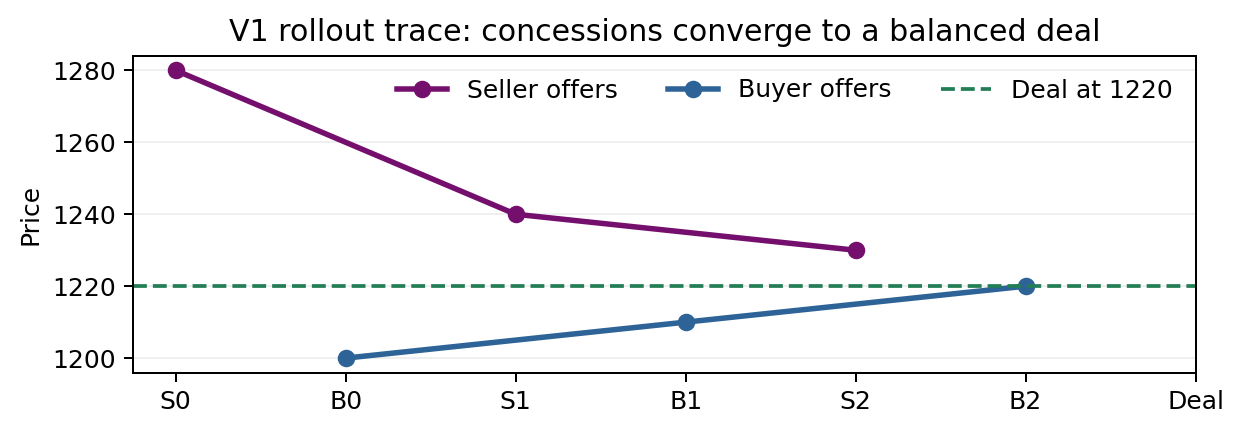
\includegraphics[width=0.85\linewidth]{figures/v1_trace_price_path.png}
\caption{A balanced V1 rollout. The final price is between the private thresholds and gives positive surplus to both sides.}
\label{fig:v1-trace}
\end{figure}

\subsection{Negative Results and Failure Analysis}

The project produced several useful failures:
\begin{itemize}
    \item \textbf{Seller-dominant equilibrium}: early stage-3 training often collapsed to prices at or near the buyer budget.
    \item \textbf{Behavioral artifacts in V1}: some trajectories still leaked floor-price language, reused SFT-style turn labels, or accepted deals too quickly.
    \item \textbf{Over-constrained optimization in V2 and V3}: stronger penalties improved intent on paper, but hurt legal deal rate and utility in practice.
\end{itemize}

These failures matter because they show that reward shaping is not monotonic. It is easy to add penalties that look reasonable locally but destabilize the overall game.

\section{Discussion}

\subsection{Novelty}

The main original contribution is not a single new RL algorithm, but a coherent system for making bilateral negotiation trainable and measurable:
\begin{itemize}
    \item a rule-generated private-value bargaining environment;
    \item a two-adapter GRPO setup for opposed roles on one base model;
    \item a staged curriculum with frozen-opponent phases;
    \item a shared-balance reward that pushes the game away from degenerate one-sided deals.
\end{itemize}

This combination is specific to the negotiation setting and was necessary to get usable results.

\subsection{Limitations}

The report should be read with three limitations in mind. First, our baselines are mainly internal ablations rather than a broad comparison against alternative RL methods such as PPO \citep{schulman2017ppo}. Second, the main evaluation is rollout-based and automatic; we do not yet have human judgments for realism or persuasiveness. Third, the behavior constraints are hand-designed and still incomplete, especially for subtle forms of private-value leakage.

\subsection{Future Work}

The most direct next steps are:
\begin{itemize}
    \item human evaluation of dialogue naturalness and bargaining realism;
    \item learned or classifier-based leakage detection;
    \item stronger opponent diversity beyond self-play between fixed buyer and seller adapters;
    \item broader baseline comparisons, including SFT-only and simpler RL variants.
\end{itemize}

\section{Conclusion}

We formulated second-hand price negotiation as a private-value RL problem for large language models and built a complete training pipeline around that formulation. The strongest result comes from a balanced GRPO stage-3 reward that keeps both parties economically viable while preserving high legal-deal rate. At the same time, the project surfaced an important negative lesson: adding more rules and penalties does not guarantee a better negotiator. In this domain, good RL performance depends on a careful balance between language quality, safety constraints, and game-theoretic incentives.

\bibliographystyle{plainnat}
\bibliography{references}

\end{document}
